\documentclass[border=8pt]{standalone}
% Shared preamble for IronClaw thesis figures (standalone TikZ).
\renewcommand{\familydefault}{\sfdefault}
\usepackage{tikz}
\usetikzlibrary{arrows.meta,positioning,calc,fit,backgrounds,shapes.geometric,shapes.misc}

% IronClaw palette (matches slides.tex)
\definecolor{IronDark}{HTML}{1A2B3C}
\definecolor{IronBlue}{HTML}{2E86AB}
\definecolor{IronTeal}{HTML}{06A77D}
\definecolor{IronOrange}{HTML}{F18F01}
\definecolor{IronRed}{HTML}{C73E1D}
\definecolor{IronLight}{HTML}{F4F7F9}
\definecolor{IronGray}{HTML}{5D6D7E}

\tikzset{
  figtitle/.style={font=\large\bfseries\color{IronDark}, align=center},
  hostbox/.style={draw=IronBlue, rounded corners=5pt, fill=IronBlue!8,
                  line width=1pt, align=center, font=\small\color{white}},
  hostfill/.style={draw=IronBlue, rounded corners=4pt, fill=IronBlue,
                   line width=0.8pt, align=center, font=\small\color{white},
                   text width=3.1cm, minimum height=0.85cm},
  guestfill/.style={draw=IronOrange, rounded corners=4pt, fill=IronOrange!85,
                    line width=0.8pt, align=center, font=\small\color{white},
                    text width=3.1cm, minimum height=0.85cm},
  guestsoft/.style={draw=IronOrange, rounded corners=4pt, fill=IronOrange!25,
                    line width=0.8pt, align=center, font=\small\color{IronDark},
                    text width=3.1cm, minimum height=0.75cm},
  arrow/.style={-{Latex[length=2.6mm,width=2mm]}, line width=0.9pt, IronDark},
  biarrow/.style={{Latex[length=2.6mm,width=2mm]}-{Latex[length=2.6mm,width=2mm]},
                  line width=0.9pt, IronDark},
  note/.style={font=\footnotesize\color{IronGray}, align=center},
}

\begin{document}
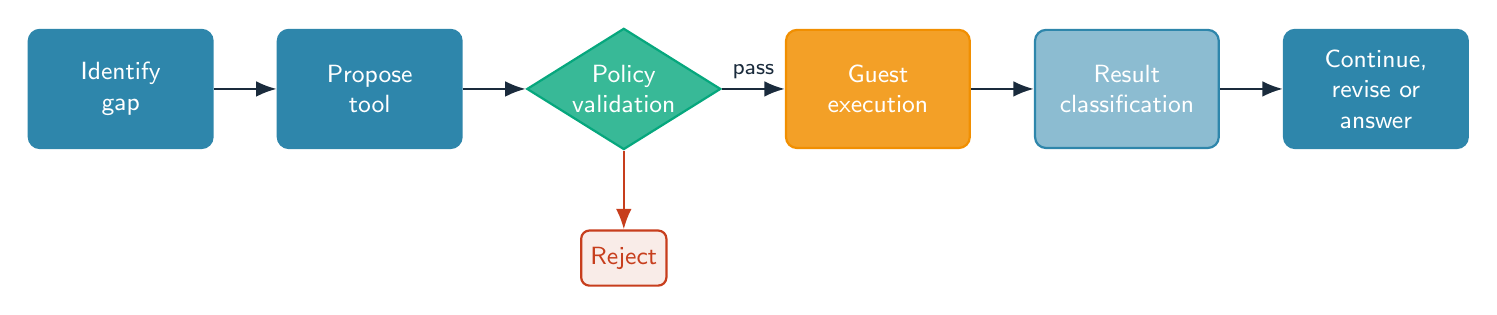
\begin{tikzpicture}[node distance=8mm]

  \tikzset{
    stage/.style={rounded corners=4pt, align=center, line width=0.8pt,
                  minimum height=1.5cm, text width=2.1cm, font=\small},
    hoststage/.style={stage, draw=IronBlue, fill=IronBlue,   text=white},
    gueststage/.style={stage, draw=IronOrange, fill=IronOrange!85, text=white},
    softstage/.style={stage, draw=IronBlue, fill=IronBlue!55, text=white},
  }

  \node[hoststage] (identify) {Identify\\gap};
  \node[hoststage, right=of identify] (propose) {Propose\\tool};
  \node[draw=IronTeal, fill=IronTeal!80, text=white, diamond, aspect=1.6,
        align=center, line width=0.8pt, font=\small, inner sep=1pt,
        right=of propose] (policy) {Policy\\validation};
  \node[gueststage, right=of policy] (exec) {Guest\\execution};
  \node[softstage, right=of exec] (classify) {Result\\classification};
  \node[hoststage, right=of classify] (answer) {Continue,\\revise or\\answer};

  \draw[arrow] (identify) -- (propose);
  \draw[arrow] (propose)  -- (policy);
  \draw[arrow] (policy)   -- node[above, note] {pass} (exec);
  \draw[arrow] (exec)     -- (classify);
  \draw[arrow] (classify) -- (answer);

  % reject path from the policy gate
  \node[draw=IronRed, fill=IronRed!10, rounded corners=3pt, line width=0.8pt,
        font=\small\color{IronRed}, minimum height=0.7cm,
        below=1.0cm of policy] (reject) {Reject};
  \draw[arrow, IronRed] (policy.south) -- (reject.north);

\end{tikzpicture}
\end{document}
